\begin{frame}[t]{Previous steps}
\begin{itemize}
  \item What do we need when compiling?
    \begin{itemize}
      \item Compile with debug information.
        \begin{itemize}
          \item Flag \cppkey{-g}: Configurations \cppid{Debug} or \cppid{RelWithDebInfo}.
        \end{itemize}
      \item Compilation flag for measuring coverage:
        \begin{itemize}
          \item Flag \cppkey{- -coverage}.
        \end{itemize}
      \item Link with coverage library:
        \begin{itemize}
          \item Library \cppkey{libgcov}.
        \end{itemize}
    \end{itemize}
\end{itemize}
\end{frame}

\begin{frame}[t,fragile]{Configuring compilation}
\begin{block}{utest/CMakeLists.txt}\tiny
\inputminted[lastline=18]{cmake}{examples/vector3/utest/CMakeLists.txt}
\end{block}
\end{frame}

\begin{frame}[t]{Tools}
\begin{itemize}
  \item \cppkey{gcov}: Basic tool for coverage annotation.
    \begin{itemize}
      \item Generates an annotated copy of source code with frequency counters.
    \end{itemize}
  \item \cppkey{lcov}: Front-end for graphical information generation from \cppkey{gcov}.
    \begin{itemize}
      \item Generates additional information including navigation.
    \end{itemize}
  \item \cppkey{genhtml}: Generates an HTML view from \cppkey{lcov} data files.
    \begin{itemize}
      \item Effective generation of hyperlinked HTML pages.
    \end{itemize}
\end{itemize}
\end{frame}

\begin{frame}[t,fragile]{Configuring generation}
\begin{block}{utest/CMakeLists.txt}\tiny
\inputminted[firstline=23]{cmake}{examples/vector3/utest/CMakeLists.txt}
\end{block}
\end{frame}

\begin{frame}[t]{Generated report}
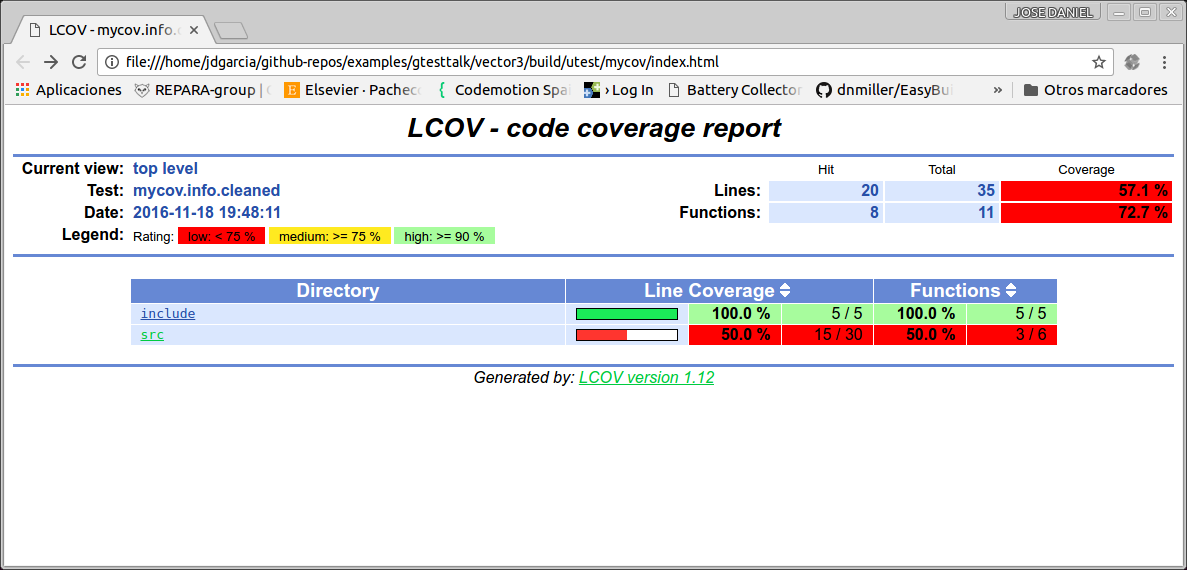
\includegraphics[width=\textwidth]{img/lcov1.png}
\end{frame}

\begin{frame}[t]{Generated report}
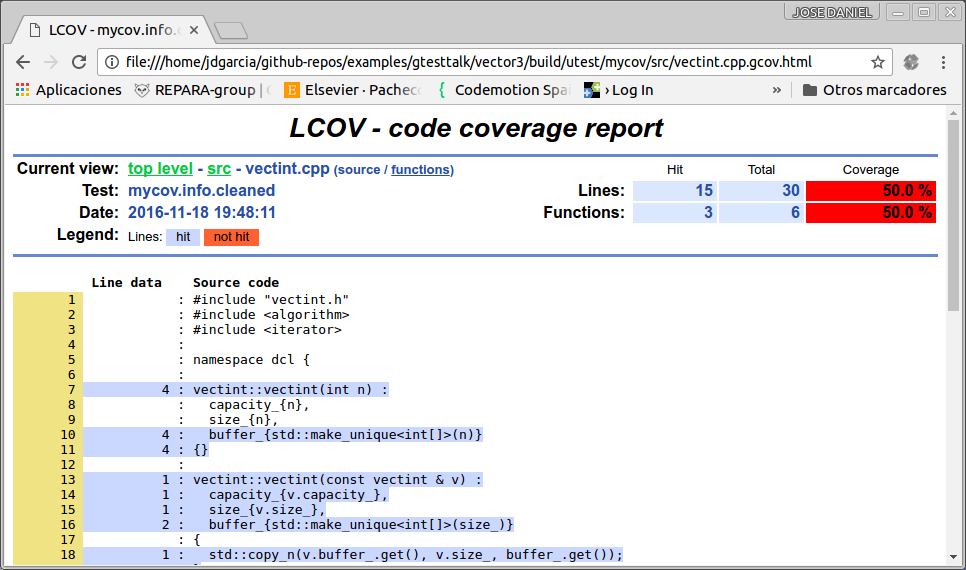
\includegraphics[width=\textwidth]{img/lcov2.png}
\end{frame}

\begin{frame}[t]{Generated report}
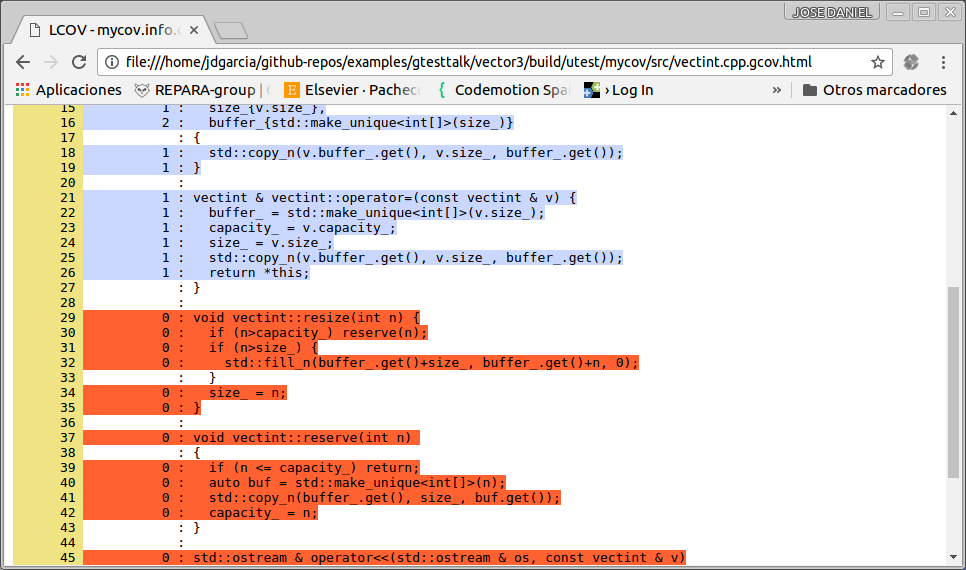
\includegraphics[width=\textwidth]{img/lcov3.png}
\end{frame}
